\documentclass[9pt,twocolumn,twoside,]{pnas-new}

% Use the lineno option to display guide line numbers if required.
% Note that the use of elements such as single-column equations
% may affect the guide line number alignment.


\usepackage[T1]{fontenc}
\usepackage[utf8]{inputenc}

% tightlist command for lists without linebreak
\providecommand{\tightlist}{%
  \setlength{\itemsep}{0pt}\setlength{\parskip}{0pt}}


% Pandoc citation processing
\newlength{\cslhangindent}
\setlength{\cslhangindent}{1.5em}
\newlength{\csllabelwidth}
\setlength{\csllabelwidth}{3em}
\newlength{\cslentryspacingunit} % times entry-spacing
\setlength{\cslentryspacingunit}{\parskip}
% for Pandoc 2.8 to 2.10.1
\newenvironment{cslreferences}%
  {}%
  {\par}
% For Pandoc 2.11+
\newenvironment{CSLReferences}[2] % #1 hanging-ident, #2 entry spacing
 {% don't indent paragraphs
  \setlength{\parindent}{0pt}
  % turn on hanging indent if param 1 is 1
  \ifodd #1
  \let\oldpar\par
  \def\par{\hangindent=\cslhangindent\oldpar}
  \fi
  % set entry spacing
  \setlength{\parskip}{#2\cslentryspacingunit}
 }%
 {}
\usepackage{calc}
\newcommand{\CSLBlock}[1]{#1\hfill\break}
\newcommand{\CSLLeftMargin}[1]{\parbox[t]{\csllabelwidth}{#1}}
\newcommand{\CSLRightInline}[1]{\parbox[t]{\linewidth - \csllabelwidth}{#1}\break}
\newcommand{\CSLIndent}[1]{\hspace{\cslhangindent}#1}


\templatetype{pnasresearcharticle}

\title{Réseau écologique des étudiants de Sherbrooke}




% Please give the surname of the lead author for the running footer
\leadauthor{}

% Please add here a significance statement to explain the relevance of your work
\significancestatement{}


\authorcontributions{}



\correspondingauthor{\textsuperscript{} }

% Keywords are not mandatory, but authors are strongly encouraged to provide them. If provided, please include two to five keywords, separated by the pipe symbol, e.g:
 \keywords{  BIO500 |  Usherbrooke |  Projet de Session  } 

\begin{abstract}

\end{abstract}

\dates{This manuscript was compiled on \today}
\doi{\url{www.pnas.org/cgi/doi/10.1073/pnas.XXXXXXXXXX}}

\begin{document}

% Optional adjustment to line up main text (after abstract) of first page with line numbers, when using both lineno and twocolumn options.
% You should only change this length when you've finalised the article contents.
\verticaladjustment{-2pt}



\maketitle
\thispagestyle{firststyle}
\ifthenelse{\boolean{shortarticle}}{\ifthenelse{\boolean{singlecolumn}}{\abscontentformatted}{\abscontent}}{}

% If your first paragraph (i.e. with the \dropcap) contains a list environment (quote, quotation, theorem, definition, enumerate, itemize...), the line after the list may have some extra indentation. If this is the case, add \parshape=0 to the end of the list environment.

\acknow{}

\section*{Auteurs}

Yuriko Archambault \textbackslash{} Marie-Ève Gagné \textbackslash{}
Juliette Larrivée \textbackslash{} Daphnée Longworth \textbackslash{}

\hypertarget{ruxe9sumuxe9}{%
\section{Résumé}\label{ruxe9sumuxe9}}

Les réseaux écologiques sont des outils qui sont pertinents pour
illustrer les liens dans les écosystèmes. Ils peuvent également être
utilisés comme réseaux de collaboration pour montrer les liens entre les
différents collaborateurs. Dans ce rapport, le réseau de collaboration
entre les étudiants en biologie de l'université de Sherbrooke a été
analysé afin de le comparer aux réseaux écologiques observés dans la
nature. Il a été montré que plusieurs similitudes entre le réseau de
collaborations des étudiants et ceux observés dans l'environnement
étaient observables. Notamment, la propension des étudiants à
retravailler avec les mêmes partenaires et celles de travailler avec
d'autres étudiants de la même cohorte et du même programme.

\begin{center}\rule{0.5\linewidth}{0.5pt}\end{center}

\hypertarget{introduction}{%
\section{Introduction}\label{introduction}}

Les réseaux écologiques permettent d'illustrer les liens entre
différentes espèces ou entre différents individus d'une même espèce ou
d'un même groupe ainsi qu'avec leur environnement. Ils sont très utiles
pour mieux comprendre les interactions dans un écosystème et peuvent
donc être d'une grande aide en conservation (Windsor et al. 2023; Delmas
et al. 2019). Ce type de réseaux est utile en écologie, mais peut
également servir à d'autres domaines, comme les sciences sociales. En
effet, les réseaux de collaborations sont pertinents pour mieux
comprendre la dynamique et les échanges dans des groupes de travail ou
dans des groupes sociaux (Lau et al. 2017). Il arrive que certains
schémas d'interactions soient observés dans plusieurs groupes d'espèces
ou plusieurs espèces dans la nature. Ainsi, ce projet s'intéresse à la
similarité entre les propriétés des réseaux écologiques naturels et
celles du réseau de collaboration chez les étudiants des différents
baccalauréats en biologie de l'université de Sherbrooke. Plus
précisément, il cherche à déterminer si les étudiants interagissent
davantage avec des étudiants du même programme qu'eux, si les étudiants
collaborent principalement avec des étudiants de la même cohorte et si
les étudiants préfèrent travailler avec les mêmes collaborateurs à
plusieurs reprises.

\hypertarget{muxe9thode}{%
\section{Méthode}\label{muxe9thode}}

La collecte des données a été réalisée auprès des étudiants inscrits
dans le cours de méthodes en écologie computationnelle (BIO500). Elle a
été effectuée sous la forme d'un fichier Excel à remplir. Ainsi, il a
été possible d'amasser des informations pertinentes sur chacun des
étudiants et sur chacune des collaborations qu'ils ont réalisées au
courant des différentes sessions et des différents cours de leurs
programmes universitaires. Trois tables distinctes ont résulté de cette
collecte de données, soit une table étudiant qui contient les
informations sur les étudiants eux-mêmes et tous ceux avec qui ils ont
collaboré soit les noms, les programmes et la cohorte. La deuxième
table, collaboration, indique toutes les interactions que l'étudiant a
eues avec d'autres étudiants au courant de son baccalauréat, le sigle du
cours dans lequel l'interaction a eu lieu et la session correspondante.
Finalement, la dernière table, cours, contient les informations sur les
sigles des cours, le nombre de crédits correspondants et si le cours est
obligatoire ou optionnel.

Par la suite, les étapes de compilations des données, d'analyses et de
rédaction du rapport ont toutes été réalisées à partir de R studio et de
certaines de ses extensions. Plus spécifiquement, un nettoyage des
données a d'abord été réalisé à partir de code R, puis les données
regroupées et nettoyées ont été injectées dans des bases de données
SQLite. Des requêtes à partir des bases de données SQLite ont permis de
répondre aux questions d'analyses. Les résultats de ses différentes
requêtes ont ensuite été convertis sous forme de graphiques et
d'illustrations à l'aide de code sur R et de certaines extensions, tel
igraph. Target a permis d'automatiser l'exécution du projet, puis le
rapport a été rédigé à l'aide de R Markdown. Le répertoire de travail a
été sauvegardé sur un dépôt GitHub.

\hypertarget{ruxe9sultats}{%
\section{Résultats}\label{ruxe9sultats}}

Illustration 1 (Yuriko): Réseau des étudiants

Les résultats obtenus montrent qu'une proportion des étudiants en
biologie de l'université de Sherbrooke préfèrent collaborer avec les
mêmes personnes. En effet, certains individus sont plutôt en retrait du
réseau et semblent collaborer avec un nombre restreint de personnes qui
sont toujours les mêmes. Il est également intéressant de noter que
certains étudiants sont liés au reste du réseau uniquement par un autre
étudiant qui a collaboré avec le reste du réseau. Aussi, les étudiants
qui se retrouvent au centre du réseau sont ceux qui ont collaboré avec
le plus grand nombre d'étudiants. Il semble y avoir une majorité
d'étudiants qui collaborent avec plusieurs personnes différentes et
quelques groupes plus en retrait.

Illustration 2 (Yuriko) : Réseau selon la cohorte

Illustration 3 (Yuriko) : Réseau selon le programme

Figure 1 : Nombre de fois qu'une paire d'étudiant va travailler ensemble

\begin{verbatim}
## 
## Attachement du package : 'dplyr'
\end{verbatim}

\begin{verbatim}
## Les objets suivants sont masqués depuis 'package:stats':
## 
##     filter, lag
\end{verbatim}

\begin{verbatim}
## Les objets suivants sont masqués depuis 'package:base':
## 
##     intersect, setdiff, setequal, union
\end{verbatim}

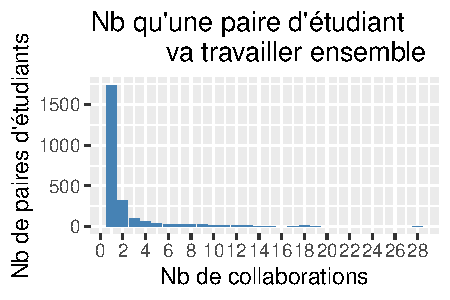
\includegraphics{Rmarkdown_Reseau_Ecologique_files/figure-latex/unnamed-chunk-2-1.pdf}

Préférence de collègue pour les étudiants. Comme illustré dans le
graphique X, la pente positive nous indique que les étudiants de
biologie semblent préférer travailler avec les mêmes étudiants. On peut
également constater que\ldots. Si on a une courbe qui va vers le haut,
oui les étudiants préfèrent travailler avec les mêmes étudiants.

\hypertarget{discussion}{%
\section{Discussion}\label{discussion}}

Dans la nature, les espèces qui cohabitent ensemble et qui ont interagi
entre elles une première fois ont une probabilité raisonnable
d'interagir ensemble si elles se rencontrent à nouveau (Delmas et al.
2019; Olesen, Stefanescu, and Traveset 2011). Ainsi, les résultats
obtenus montrent que les étudiants en biologie de l'université de
Sherbrooke ont un comportement similaire. En effet, la figure X permet
d'observer que la majorité des élèves ont collaboré plus d'une fois avec
les mêmes personnes. Aussi, dans cette situation, on peut considérer que
les étudiants d'un même programme ou d'une même cohorte sont des
individus qui cohabitent ensemble. Cette situation est plutôt logique.
En effet, les étudiants ayant collaboré avec une personne dans le passé
qui ont été satisfaits du fruit de cette collaboration ont avantage à
refaire une collaboration avec cette même personne, car ils savent à
quoi s'attendre, ils sont donc confiants par rapport au résultat de la
collaboration. Aussi, les résultats obtenus montrent que les étudiants
d'un même programme vont collaborer plus souvent avec des individus qui
proviennent du même programme qu'eux (figure X). De ce fait, on peut
faire le parallèle avec les individus d'une même espèce. Dans la nature,
les individus ont tendance à interagirent plus fréquemment avec des
individus de la même espèce qu'eux lorsqu'il s'agit d'une espèce
grégaire (Poisot and Gravel 2014; Lau et al. 2017; Landi et al. 2018).
En outre, les étudiants semblent avoir un comportement similaire si le
programme d'étude est considéré comme une espèce. Cette tendance que les
élèves ont de collaborer avec d'autres étudiants issus du même programme
d'étude pourrait s'expliquer de plusieurs façons. D'abord, comme énoncé
plus haut, il est plus simple de collaborer avec des individus que nous
connaissons déjà. Ensuite, les étudiants pourraient vouloir collaborer
avec d'autres étudiants du même programme qu'eux même, et ce même s'ils
n'ont jamais collaboré auparavant, car ils ont des connaissances
similaires. Ainsi, ils peuvent se fier que la personne aura des
aptitudes semblables pour réaliser le projet.

\hypertarget{conclusion}{%
\section{Conclusion}\label{conclusion}}

Somme toute, il est possible de constater qu'il y a certaines
ressemblances entre les réseaux écologiques et le réseau de
collaboration entre les étudiants de biologie. En effet, comme observé
en nature, il est possible de constater une tendance chez certains
étudiants de collaborer avec les mêmes personnes à plusieurs reprises.
De plus, les étudiants d'une même cohorte et d'un même programme
collaborent plus souvent entre eux. Ces similitudes entre les réseaux
écologiques et le réseau de collaboration des étudiants permettent de se
demander si, peu importe l'espèce, tous les animaux ont une certaine
tendance à rechercher la collaboration de ceux qui les ressemblent le
plus.

\hypertarget{bibliographie}{%
\section{Bibliographie}\label{bibliographie}}

\hypertarget{figure-et-tableau}{%
\section{Figure et tableau}\label{figure-et-tableau}}

\begin{figure}
\centering
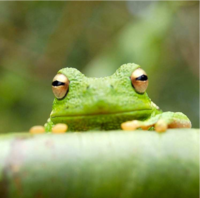
\includegraphics{frog.png}
\caption{Nom de la figure.}
\end{figure}

\hypertarget{refs}{}
\begin{CSLReferences}{1}{0}
\leavevmode\vadjust pre{\hypertarget{ref-Delmas2019}{}}%
Delmas, Eva, Mathilde Besson, Marie-Hélène Brice, Laura A Burkle, Giulio
V Dalla Riva, Marie-Josée Fortin, Dominique Gravel, et al. 2019.
{``Analysing Ecological Networks of Species Interactions.''}
\emph{Biological Reviews} 94 (1): 16--36.

\leavevmode\vadjust pre{\hypertarget{ref-Landi2018}{}}%
Landi, Pietro, Henintsoa O Minoarivelo, Åke Brännström, Cang Hui, and
Ulf Dieckmann. 2018. {``Complexity and Stability of Ecological Networks:
A Review of the Theory.''} \emph{Population Ecology} 60: 319--45.

\leavevmode\vadjust pre{\hypertarget{ref-Lau2017}{}}%
Lau, Matthew K, Stuart R Borrett, Benjamin Baiser, Nicholas J Gotelli,
and Aaron M Ellison. 2017. {``Ecological Network Metrics: Opportunities
for Synthesis.''} \emph{Ecosphere} 8 (8): e01900.

\leavevmode\vadjust pre{\hypertarget{ref-Olesen2011}{}}%
Olesen, Jens M, Constantí Stefanescu, and Anna Traveset. 2011.
{``Strong, Long-Term Temporal Dynamics of an Ecological Network.''}
\emph{PloS One} 6 (11): e26455.

\leavevmode\vadjust pre{\hypertarget{ref-Poisot2014}{}}%
Poisot, Timothée, and Dominique Gravel. 2014. {``When Is an Ecological
Network Complex? Connectance Drives Degree Distribution and Emerging
Network Properties.''} \emph{PeerJ} 2: e251.

\leavevmode\vadjust pre{\hypertarget{ref-Windsor2023}{}}%
Windsor, Fredric M, Johan van den Hoogen, Thomas W Crowther, and Darren
M Evans. 2023. {``Using Ecological Networks to Answer Questions in
Global Biogeography and Ecology.''} \emph{Journal of Biogeography} 50
(1): 57--69.

\end{CSLReferences}



% Bibliography
% \bibliography{pnas-sample}

\end{document}
